\chapter{Before Transformer}
\label{ch:before-transformer}

\section{Why Start Here?}

In 2014, a Google research team demonstrated that a neural translation model could translate a 30-word sentence by compressing it into a single 1{,}000-dimensional vector, then expanding that vector back into the target language. It worked---astonishingly well, by the standards of the time---but the approach had an absurd limitation: the 5th word and the 25th word of the source sentence had to compete for space in the same fixed-size vector. By 2017, this bottleneck was gone, replaced by an architecture---the Transformer---that let every output word look directly at every input word. The shift took only three years, but the ideas behind it had been building for two decades.

Every design decision in \emph{Attention Is All You Need}~\cite{vaswani2017attention} was a direct response to limitations that researchers had struggled with throughout those decades: the inability of count-based models with fixed context windows to capture long-range dependencies, the sequential bottleneck of recurrent networks, and the fragility of early attention mechanisms bolted onto encoder--decoder pipelines.

This chapter traces the arc from counting-based language models through neural sequence models to the point where the field was ready for a fully attention-based architecture. The goal is not historical completeness but \emph{architectural intuition}: by the end of this chapter, you should be able to articulate exactly which problems each generation solved and which problems it left open.

\subsection*{Learning Objectives}

After completing this chapter, you should be able to:

\begin{enumerate}
    \item Derive the $n$-gram language modeling objective from the chain rule and explain why sparsity makes raw counts fail.
    \item Explain why distributed representations (Word2Vec, GloVe) solve the generalization problem but not the context problem.
    \item Describe how RNN, LSTM, and GRU process sequences, and trace the gradient flow that causes vanishing/exploding gradients.
    \item Explain the Seq2Seq bottleneck and how Bahdanau attention resolves it.
    \item Articulate why recurrent architectures cannot be parallelized across time steps, and why this limitation made the Transformer necessary for large-scale pretraining.
\end{enumerate}

\subsection*{Notation}

The following conventions are used throughout this chapter and the rest of the book:

\begin{center}
\begin{tabular}{ll}
\toprule
Symbol & Meaning \\
\midrule
$w_t$ & The token (word or character) at position $t$ \\
$\mathbf{x}_t$ & The embedding vector for token $w_t$ \\
$\mathbf{h}_t$ & Hidden state at time step $t$ \\
$\mathbf{c}_t$ & LSTM cell state at time step $t$ \\
$\mathbf{a}_t$ & Attention context vector at decoder step $t$ \\
$\odot$ & Elementwise (Hadamard) product \\
$[\mathbf{a}; \mathbf{b}]$ & Concatenation of vectors $\mathbf{a}$ and $\mathbf{b}$ \\
$\sigma(\cdot)$ & Logistic sigmoid function \\
$e_{t,s}$ & Alignment score (decoder step $t$, encoder position $s$) \\
$\alpha_{t,s}$ & Attention weight (softmax-normalized alignment score) \\
$|V|$ & Vocabulary size \\
$T$ & Sequence length \\
PPL & Perplexity \\
\bottomrule
\end{tabular}
\end{center}

\subsection*{Timeline}

The following table situates the key contributions covered in this chapter. Notice how the pace accelerated: the gap between $n$-grams and neural LMs was a decade, but the gap between Seq2Seq and the Transformer was only three years.

\begin{center}
\begin{tabularx}{\textwidth}{@{}lp{3.8cm}X@{}}
\toprule
Year & Contribution & Key idea \\
\midrule
1990s & $N$-gram LMs & Autoregressive factorization; count-based estimation \\
1997 & LSTM & Gated cell state to mitigate vanishing gradients \\
2003 & Neural LM (Bengio) & Learned embeddings + feedforward next-word prediction \\
2013 & Word2Vec & Efficient training of distributional word vectors \\
2014 & GloVe & Word vectors from global co-occurrence statistics \\
2014 & GRU & Simplified gating (2 gates instead of 3) \\
2014 & Seq2Seq & Encoder--decoder RNN for sequence transduction \\
2015 & Bahdanau attention & Dynamic, position-dependent context vector \\
2015 & Luong attention & Dot-product scoring $\to$ faster, simpler \\
2017 & Transformer & Self-attention replaces recurrence entirely \\
2018 & ELMo & Pretrained contextualized representations from biLSTM \\
\bottomrule
\end{tabularx}
\end{center}

\section{N-gram Language Models}

A language model assigns a probability to a sequence of tokens. The simplest approach is to estimate this probability from counts.

\subsection{The Chain Rule and Markov Assumption}

The probability of a sequence $w_1, w_2, \ldots, w_T$ can be decomposed exactly via the chain rule of probability:
\[
P(w_1, w_2, \ldots, w_T) = \prod_{t=1}^{T} P(w_t \mid w_1, \ldots, w_{t-1}).
\]
This decomposition is exact but intractable: the conditioning context grows with every token, and most contexts will never appear in any finite corpus. The \emph{Markov assumption} truncates the context to a fixed window of $n-1$ tokens:
\[
P(w_t \mid w_1, \ldots, w_{t-1}) \approx P(w_t \mid w_{t-n+1}, \ldots, w_{t-1}).
\]
An $n$-gram model estimates each conditional probability by counting:
\[
P(w_t \mid w_{t-n+1}, \ldots, w_{t-1}) = \frac{\text{count}(w_{t-n+1}, \ldots, w_t)}{\text{count}(w_{t-n+1}, \ldots, w_{t-1})}.
\]

\paragraph{A concrete example.}
Consider a tiny corpus of three sentences: ``the cat sat,'' ``the cat ran,'' and ``the dog sat.'' A bigram model estimates:

\begin{center}
\begin{tabular}{lcc}
\toprule
Bigram & Count & $P(w_t \mid w_{t-1})$ \\
\midrule
(the, cat) & 2 & $2/3$ \\
(the, dog) & 1 & $1/3$ \\
(cat, sat) & 1 & $1/2$ \\
(cat, ran) & 1 & $1/2$ \\
(dog, sat) & 1 & $1/1$ \\
\bottomrule
\end{tabular}
\end{center}

Now suppose we want to score the sentence ``the dog ran.'' The bigram (dog, ran) has count 0, so $P(\text{ran} \mid \text{dog}) = 0$ and the entire sentence probability is zero---even though both ``dog'' and ``ran'' are known words. This is the sparsity problem: raw counts cannot generalize to unseen but plausible combinations.

We can also compute the perplexity of a sentence the model \emph{has} seen. For ``the cat sat'' (treating ``the'' as given):
\[
\text{PPL} = \exp\!\Bigl(-\tfrac{1}{2}\bigl[\log P(\text{cat}\mid\text{the}) + \log P(\text{sat}\mid\text{cat})\bigr]\Bigr) = \exp\!\Bigl(-\tfrac{1}{2}[\log\tfrac{2}{3} + \log\tfrac{1}{2}]\Bigr) \approx 1.73.
\]
Low perplexity indicates the model is confident and correct. A random baseline over a 5-word vocabulary would give $\text{PPL} = 5$.

\subsection{Smoothing and Sparsity}

Raw counts produce zero probabilities for any $n$-gram not observed in training data. This is not an edge case---even with billions of tokens, most valid 5-grams will never appear. Smoothing techniques address this:

\begin{itemize}
    \item \textbf{Add-$k$ smoothing} adds a small constant to every count, but distorts the distribution uniformly regardless of context.
    \item \textbf{Kneser--Ney smoothing} uses a discount on observed counts and redistributes probability mass based on how many distinct contexts a word appears in, which provides a much better estimate for rare events.
    \item \textbf{Backoff and interpolation} combine estimates from different orders: when the 5-gram count is zero, fall back to the 4-gram, then the 3-gram, and so on.
\end{itemize}

Despite these techniques, $n$-gram models face a fundamental scaling problem: the number of possible $n$-grams grows as $|V|^n$, where $|V|$ is the vocabulary size. Increasing $n$ beyond 5 or 6 becomes impractical, which means the model can never capture dependencies longer than a few words.

\subsection{What N-grams Taught Us}

N-gram models established two ideas that persist in modern language modeling:

\begin{enumerate}
    \item \textbf{Autoregressive factorization.} Decomposing sequence probability into a product of conditional next-token probabilities is the foundation of GPT-style models.
    \item \textbf{Perplexity as evaluation.} Perplexity---the exponentiated average negative log-likelihood---remains the standard intrinsic metric for language models:
    \[
    \text{PPL} = \exp\!\left(-\frac{1}{T}\sum_{t=1}^T \log P(w_t \mid w_{<t})\right).
    \]
    A common confusion is whether the quantity inside the exponent is \emph{entropy}. Strictly, it is the \emph{empirical cross-entropy} $H(p, q)$ between the data distribution $p$ and the model distribution $q$. Cross-entropy decomposes as $H(p, q) = H(p) + D_{\text{KL}}(p \,\|\, q)$, so it equals the true entropy of language only when the model is perfect ($D_{\text{KL}} = 0$). In practice, perplexity measures how well the model fits the data, not an intrinsic property of language itself. A PPL of 30 means the model is, on average, as uncertain as if it were choosing uniformly among 30 candidates at each step.
\end{enumerate}

What $n$-grams could not do is generalize: ``the cat sat on the mat'' and ``the dog sat on the rug'' share no information under a bigram model because the tokens are different. Bridging this gap requires learning distributed representations.

\medskip
\noindent\fbox{\parbox{\dimexpr\textwidth-2\fboxsep-2\fboxrule\relax}{\textbf{Pause and verify.} Suppose you increase a bigram model to a 10-gram model. Does this solve the sparsity problem, the generalization problem, both, or neither? Think carefully before reading on.}}
\medskip

\begin{quickrecap}
\textbf{Quick Recap.}
\begin{itemize}[nosep,leftmargin=1.5em]
  \item N-grams use the chain rule + counting; they established autoregressive factorization and perplexity.
  \item Fundamental limit: unseen n-grams get zero probability---discrete tokens share no information.
  \item No amount of smoothing fixes the generalization gap.
\end{itemize}
\end{quickrecap}

\section{Distributed Word Representations}

\subsection{From Counts to Vectors}

The core insight of neural language modeling is that words should be represented as dense vectors in a continuous space, where proximity encodes semantic similarity. Two words that appear in similar contexts should have similar representations, even if they never co-occur directly.

Bengio et al.~\cite{bengio2003neural} proposed the first neural language model: a feedforward network that takes the embeddings of the previous $n-1$ words, concatenates them, passes them through a hidden layer, and produces a distribution over the next word. This model could generalize across similar contexts because similar words had similar embeddings. However, it was slow to train and still limited to a fixed context window.

\subsection{Word2Vec}

Mikolov et al.~\cite{mikolov2013efficient} showed that high-quality word embeddings could be trained efficiently using two simplified architectures:

\begin{itemize}
    \item \textbf{Skip-gram:} given a center word, predict the surrounding context words. The objective maximizes:
    \[
    \sum_{t=1}^{T} \sum_{-c \leq j \leq c,\, j \neq 0} \log P(w_{t+j} \mid w_t),
    \]
    where $c$ is the context window size.
    \item \textbf{CBOW (Continuous Bag of Words):} given the context words, predict the center word.
\end{itemize}

Both models use a single linear projection followed by a softmax (or, in practice, negative sampling or hierarchical softmax to avoid computing the full vocabulary normalization). The key contribution was demonstrating that the resulting embedding space captured relational structure: the famous ``king $-$ man $+$ woman $\approx$ queen'' analogy.

\subsection{GloVe}

Pennington et al.~\cite{pennington2014glove} took a different approach with GloVe (Global Vectors for Word Representation). Instead of predicting context words from a sliding window, GloVe factorizes the global word--word co-occurrence matrix. The objective minimizes:
\[
\sum_{i,j=1}^{|V|} f(X_{ij})\,\bigl(\mathbf{w}_i^\top \tilde{\mathbf{w}}_j + b_i + \tilde{b}_j - \log X_{ij}\bigr)^2,
\]
where $X_{ij}$ is the co-occurrence count, $f$ is a weighting function that caps the influence of very frequent pairs, and $\mathbf{w}_i$, $\tilde{\mathbf{w}}_j$ are word and context vectors.

GloVe and Word2Vec produce embeddings of comparable quality. The important takeaway is conceptual: words can be meaningfully represented as points in a learned vector space, and this representation transfers across tasks. Every neural language model since---including every Transformer---begins by mapping tokens to dense embeddings.

\begin{figure}[h]
\centering
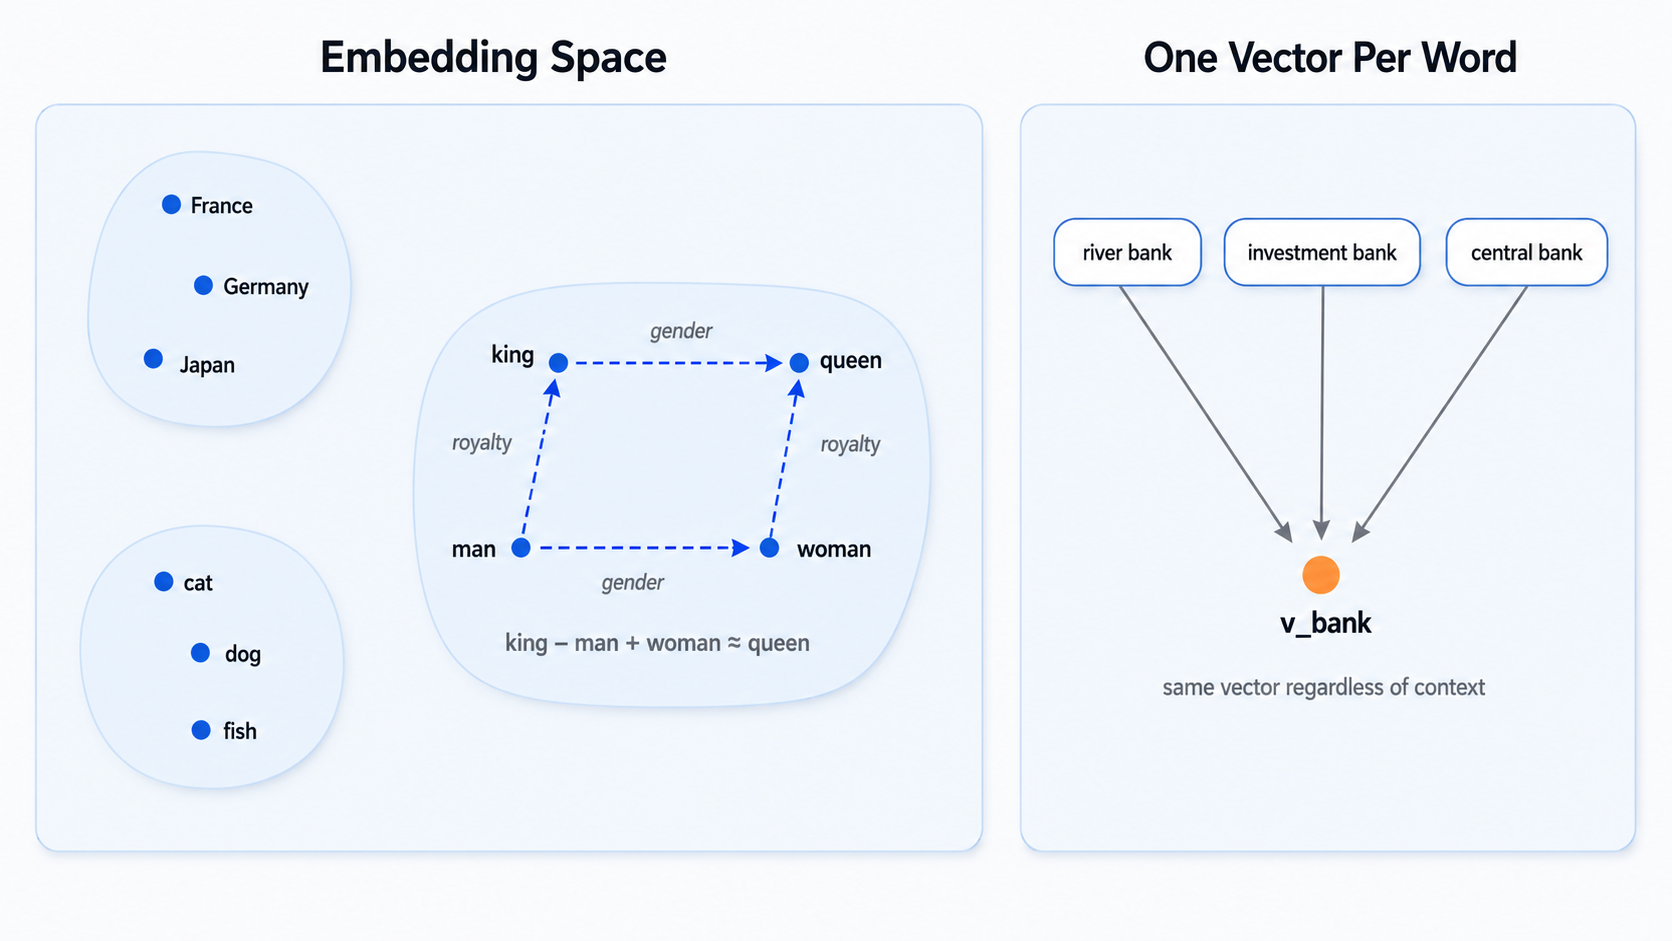
\includegraphics[width=0.9\textwidth]{figures/ch01/word2vec_embedding_space.png}
\caption{Static word embeddings capture semantic structure but collapse polysemy. \textbf{Left:} The embedding space organizes words into semantic clusters (countries, animals) and encodes relational structure---the vector offset from \emph{man} to \emph{woman} is approximately parallel to \emph{king} to \emph{queen}. \textbf{Right:} However, each word type maps to exactly one point regardless of context. All occurrences of ``bank''---whether near ``river,'' ``investment,'' or ``central''---share the single vector $\mathbf{v}_{\text{bank}}$. This polysemy problem motivates the contextual representations introduced in \S\ref{sec:contextual-preview}.}
\label{fig:word2vec-embedding}
\end{figure}

\subsection{Limitations of Static Embeddings}

Both Word2Vec and GloVe produce a single vector per word type. This means ``bank'' in ``river bank'' and ``bank'' in ``investment bank'' share the same representation. A common source of confusion is that Word2Vec's \emph{training} clearly uses context---skip-gram predicts surrounding words, CBOW predicts the center word from its neighbors. But the representation function it learns is simply $f(w) = \mathbf{v}_w$: one fixed vector per word type, regardless of sentence context. All training examples containing ``bank''---whether near ``river'' or near ``loan''---update the same vector, producing a single point that averages over all senses. In short: \emph{Word2Vec is contextual in its training signal, but static in its representation function.} Resolving this ambiguity requires \emph{contextualized} representations---embeddings that depend on the surrounding sentence.

\subsection{Preview: Contextualized Representations}
\label{sec:contextual-preview}

Static embeddings cannot adapt to sentence context---but this limitation was eventually solved by using sequence-model hidden states as word representations. To understand how, we first need to cover recurrent neural networks and LSTMs; we return to this idea in \S\ref{sec:elmo} after introducing the required machinery.

\begin{quickrecap}
\textbf{Quick Recap.}
\begin{itemize}[nosep,leftmargin=1.5em]
  \item Dense vectors solve generalization: similar words get similar representations.
  \item Word2Vec/GloVe are contextual in training signal but static in output---one fixed vector per word type.
  \item ``Bank'' near ``river'' and near ``loan'' map to the same point; fixing this requires sentence-conditioned representations.
\end{itemize}
\end{quickrecap}

\section{Recurrent Neural Networks}

\subsection{The Recurrence Idea}

Distributed representations solve the generalization problem: similar words get similar vectors, so the model can transfer knowledge across contexts. But they do not solve the \emph{context} problem. A feedforward network over embeddings still has a fixed window. To process sequences of arbitrary length, we need a different computational structure.

A recurrent neural network (RNN) processes a sequence one token at a time, maintaining a hidden state $\mathbf{h}_t$ that summarizes everything seen so far.

\begin{figure}[ht]
\centering
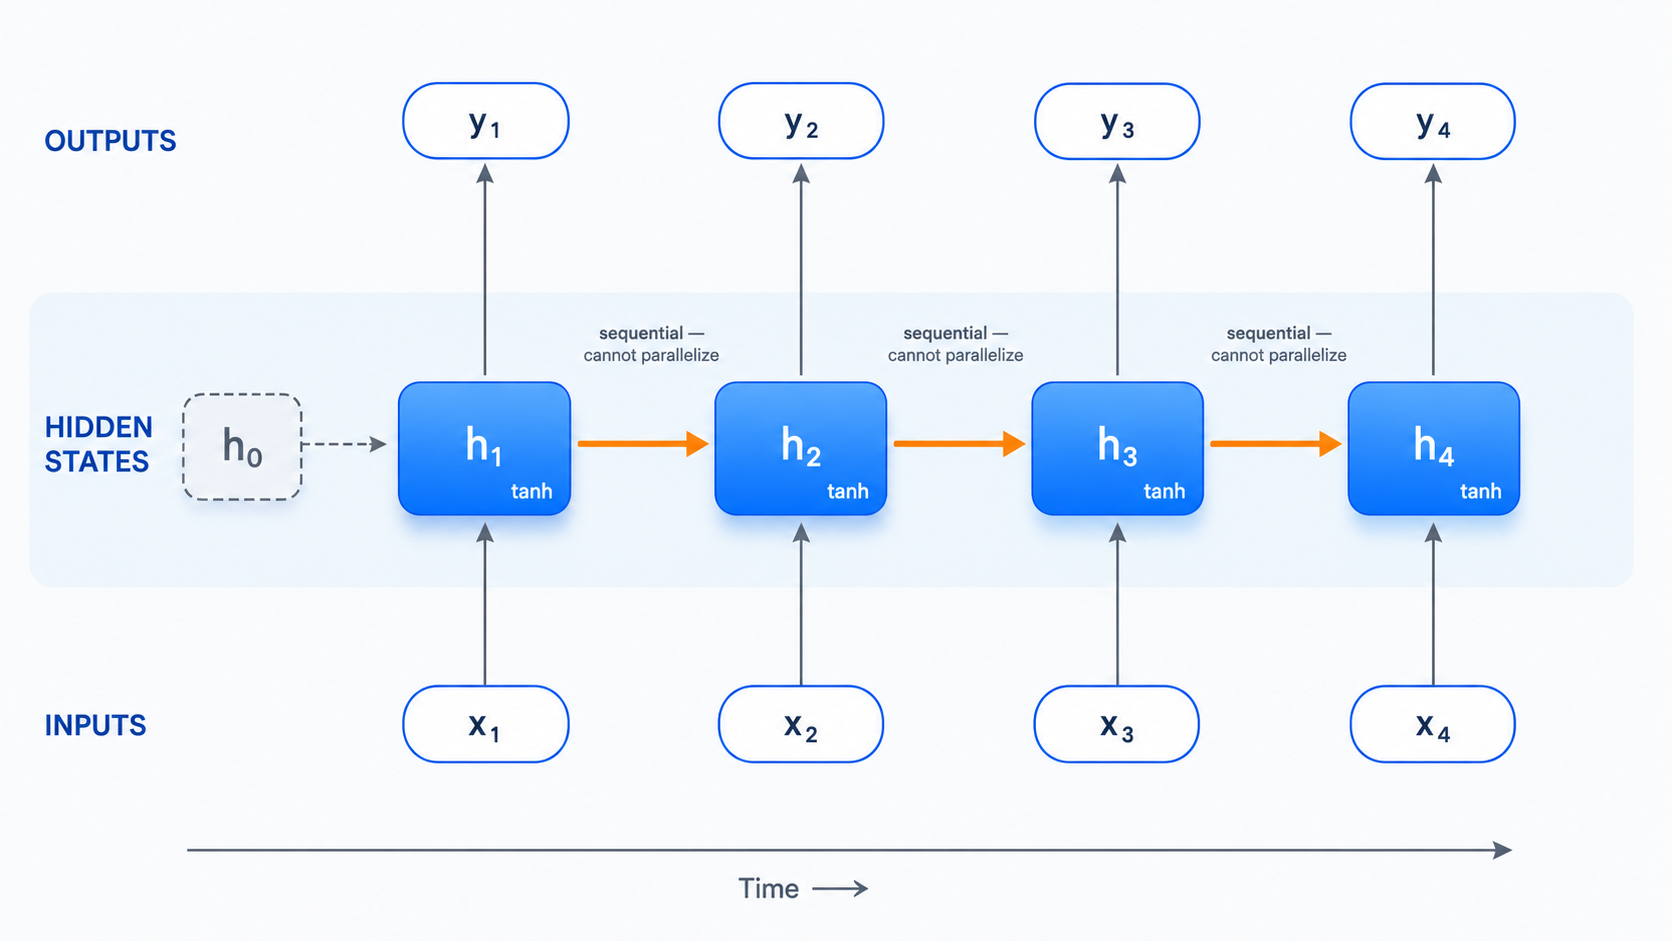
\includegraphics[width=0.85\textwidth]{figures/ch01/rnn_unrolled.png}
\caption{An RNN unrolled across $T$ time steps. The horizontal arrows between hidden states are not decorative---they represent a strict sequential dependency that prevents any parallelization across time. Computing $\mathbf{h}_4$ requires $\mathbf{h}_3$, which requires $\mathbf{h}_2$, and so on. This is the fundamental bottleneck that the Transformer eliminates.}
\label{fig:rnn-unrolled}
\end{figure}

At each step:
\[
\mathbf{h}_t = \sigma(\mathbf{W}_h \mathbf{h}_{t-1} + \mathbf{W}_x \mathbf{x}_t + \mathbf{b}),
\]
where $\mathbf{x}_t$ is the input embedding at step $t$ and $\sigma$ is a nonlinearity (typically $\tanh$). The hidden state is the model's ``memory''---unlike the fixed-length context of an $n$-gram, the hidden state is updated incrementally and can, in principle, summarize unbounded history. At each step, the model can produce an output---for language modeling, a distribution over the next token:
\[
P(w_{t+1} \mid w_{\leq t}) = \text{softmax}(\mathbf{W}_o \mathbf{h}_t + \mathbf{b}_o).
\]

Unlike $n$-gram models, an RNN has no fixed context window: in principle, $\mathbf{h}_t$ can encode information from arbitrarily far back. In practice, this does not work.

\subsection{The Vanishing and Exploding Gradient Problem}

Training an RNN requires backpropagation through time (BPTT): unrolling the recurrence for $T$ steps and computing gradients through the entire chain. The gradient of the loss at step $T$ with respect to the hidden state at step $t$ involves a product of Jacobians:
\[
\frac{\partial \mathbf{h}_T}{\partial \mathbf{h}_t} = \prod_{k=t+1}^{T} \frac{\partial \mathbf{h}_k}{\partial \mathbf{h}_{k-1}}.
\]
If the spectral radius of $\frac{\partial \mathbf{h}_k}{\partial \mathbf{h}_{k-1}}$ is consistently less than 1, this product shrinks exponentially (\emph{vanishing gradients}): the model cannot learn long-range dependencies because the error signal from distant tokens is effectively zero by the time it reaches early time steps. If the spectral radius is consistently greater than 1, the product explodes (\emph{exploding gradients}), causing numerical instability.

Gradient clipping can mitigate explosion, but vanishing gradients require architectural changes.

\medskip
\noindent\fbox{\parbox{\dimexpr\textwidth-2\fboxsep-2\fboxrule\relax}{\textbf{Intuition checkpoint.} The gradient product $\prod_{k=t+1}^{T} \frac{\partial \mathbf{h}_k}{\partial \mathbf{h}_{k-1}}$ involves repeated multiplication by the same weight matrix. How is this analogous to computing $A^n$ for a matrix $A$? What determines whether $A^n$ shrinks, explodes, or stays stable? (Hint: eigenvalues.)}}
\medskip

\subsection{LSTM}

The Long Short-Term Memory network~\cite{hochreiter1997lstm} introduces a gated cell state $\mathbf{c}_t$ that information can flow through with minimal transformation:

\begin{align}
\mathbf{f}_t &= \sigma(\mathbf{W}_f [\mathbf{h}_{t-1}, \mathbf{x}_t] + \mathbf{b}_f) & \text{(forget gate)} \\
\mathbf{i}_t &= \sigma(\mathbf{W}_i [\mathbf{h}_{t-1}, \mathbf{x}_t] + \mathbf{b}_i) & \text{(input gate)} \\
\tilde{\mathbf{c}}_t &= \tanh(\mathbf{W}_c [\mathbf{h}_{t-1}, \mathbf{x}_t] + \mathbf{b}_c) & \text{(candidate)} \\
\mathbf{c}_t &= \mathbf{f}_t \odot \mathbf{c}_{t-1} + \mathbf{i}_t \odot \tilde{\mathbf{c}}_t & \text{(cell update)} \\
\mathbf{o}_t &= \sigma(\mathbf{W}_o [\mathbf{h}_{t-1}, \mathbf{x}_t] + \mathbf{b}_o) & \text{(output gate)} \\
\mathbf{h}_t &= \mathbf{o}_t \odot \tanh(\mathbf{c}_t) & \text{(hidden state)}
\end{align}

\begin{figure}[ht]
\centering
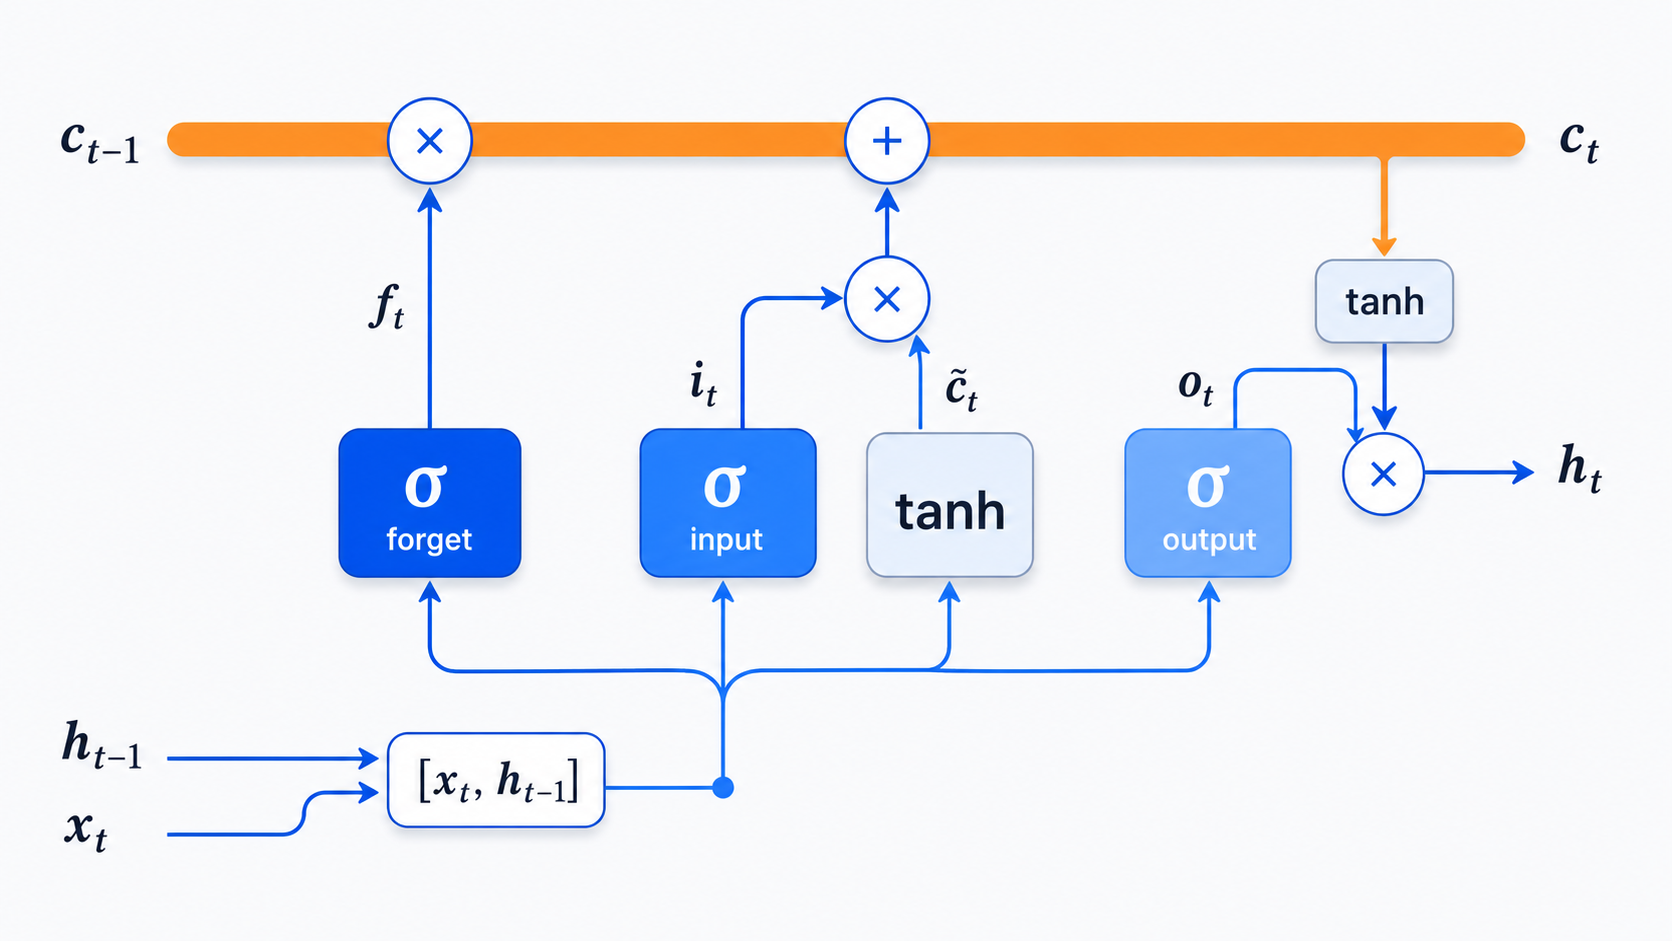
\includegraphics[width=0.85\textwidth]{figures/ch01/lstm_cell.png}
\caption{The LSTM cell. The cell state $\mathbf{c}_t$ flows horizontally with only elementwise operations (multiply by forget gate, add from input gate), creating a gradient highway that mitigates vanishing gradients.}
\label{fig:lstm-cell}
\end{figure}

The key mechanism is the \emph{forget gate} $\mathbf{f}_t$: when it is close to 1, the cell state $\mathbf{c}_{t-1}$ passes through almost unchanged. To see why this matters for gradient flow, consider the Jacobian of the cell update along the direct cell-state path: $\partial \mathbf{c}_t / \partial \mathbf{c}_{t-1}$ contains $\operatorname{diag}(\mathbf{f}_t)$. When $\mathbf{f}_t \approx \mathbf{1}$, this Jacobian is approximately the identity, so the gradient of the loss with respect to $\mathbf{c}_{t-k}$ passes through $k$ time steps without the repeated shrinkage that plagues vanilla RNNs. This is why the cell state is called a \emph{gradient highway}: it provides a near-identity path through time that allows error signals to reach early time steps intact.

\medskip
\noindent\fbox{\parbox{\dimexpr\textwidth-2\fboxsep-2\fboxrule\relax}{\textbf{Intuition checkpoint.} The forget gate outputs values in $[0, 1]$:
\[
\mathbf{f}_t = \sigma\!\bigl(\mathbf{W}_f [\mathbf{h}_{t-1}; \mathbf{x}_t] + \mathbf{b}_f\bigr).
\]
If $\mathbf{f}_t \approx \mathbf{1}$ for all time steps, what does the LSTM reduce to? If $\mathbf{f}_t \approx \mathbf{0}$, what information is lost?}}
\medskip The input gate controls what new information enters the cell, and the output gate controls what is exposed to the rest of the network. It is worth emphasizing that these gates are not hand-designed rules---they are \emph{differentiable control functions} whose parameters are learned indirectly through the prediction loss. During training, if the forget gate discards information that turns out to be needed for a later prediction, the resulting loss gradient adjusts $\mathbf{W}_f$ so that similar information is more likely to be retained in the future. The gates learn \emph{what} to remember, write, and expose entirely from the supervisory signal of next-token prediction.

LSTMs were the dominant architecture for sequence modeling from roughly 2014 to 2017. They achieved state-of-the-art results on machine translation, language modeling, speech recognition, and many other tasks.

\subsection{GRU}

The Gated Recurrent Unit~\cite{cho2014learning} simplifies the LSTM by merging the cell state and hidden state and using only two gates:

\begin{align}
\mathbf{z}_t &= \sigma(\mathbf{W}_z [\mathbf{h}_{t-1}, \mathbf{x}_t]) & \text{(update gate)} \\
\mathbf{r}_t &= \sigma(\mathbf{W}_r [\mathbf{h}_{t-1}, \mathbf{x}_t]) & \text{(reset gate)} \\
\tilde{\mathbf{h}}_t &= \tanh(\mathbf{W} [\mathbf{r}_t \odot \mathbf{h}_{t-1}, \mathbf{x}_t]) & \text{(candidate)} \\
\mathbf{h}_t &= (1 - \mathbf{z}_t) \odot \mathbf{h}_{t-1} + \mathbf{z}_t \odot \tilde{\mathbf{h}}_t & \text{(hidden state)}
\end{align}

The key difference from LSTM is structural: GRU has no separate cell state. The update gate $\mathbf{z}_t$ simultaneously decides what to forget from the old state and what to accept from the candidate---effectively merging the LSTM's forget and input gates into a single mechanism. The reset gate $\mathbf{r}_t$ controls how much of the previous hidden state feeds into the candidate computation, allowing the model to ``start fresh'' when appropriate.

Because there are only two gates instead of three and no separate cell state, GRUs have roughly 25\% fewer parameters than an equivalently-sized LSTM. In practice, GRUs and LSTMs perform comparably on most benchmarks; GRUs tend to train faster and are often preferred when data or compute is limited, while LSTMs sometimes have a slight edge on tasks requiring very precise long-range memory.

\begin{figure}[h]
\centering
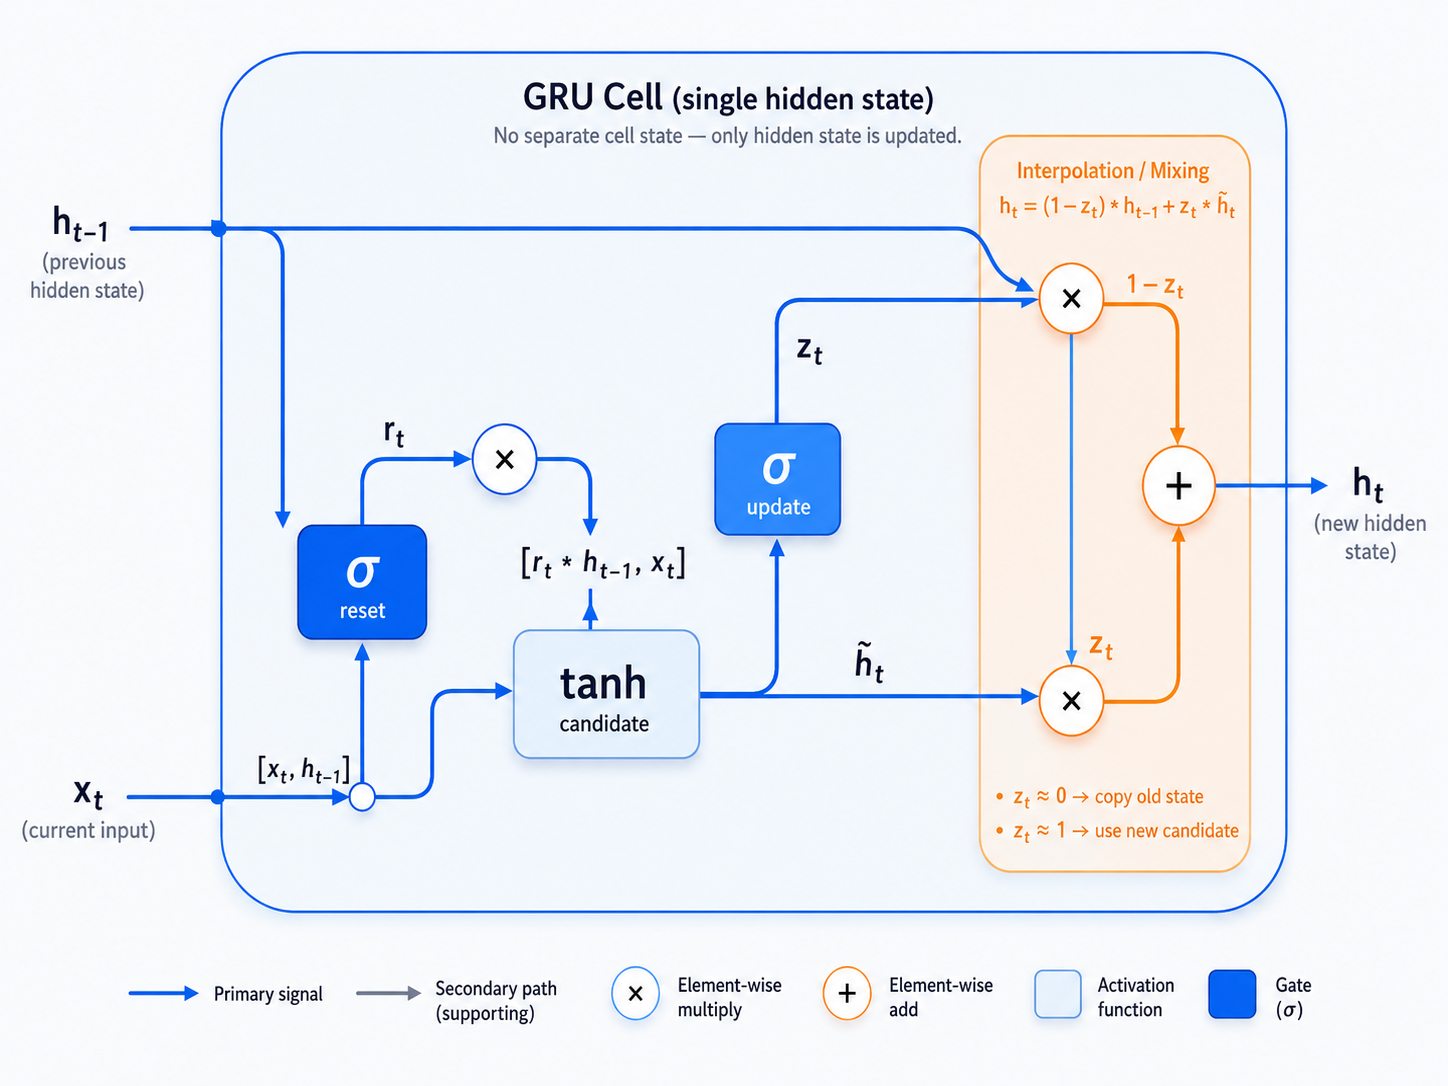
\includegraphics[width=0.85\textwidth]{figures/ch01/gru_cell.png}
\caption{GRU cell internals. Unlike the LSTM (Figure~\ref{fig:lstm-cell}), there is no separate cell state---the hidden state $\mathbf{h}_t$ serves as both memory and output. The update gate $\mathbf{z}_t$ controls the interpolation between the previous state $\mathbf{h}_{t-1}$ and the candidate $\tilde{\mathbf{h}}_t$, merging the roles of the LSTM's forget and input gates into a single mechanism.}
\label{fig:gru}
\end{figure}

\medskip
\noindent\fbox{\parbox{\dimexpr\textwidth-2\fboxsep-2\fboxrule\relax}{\textbf{Pause and verify.} The LSTM cell state $\mathbf{c}_t$ acts as a ``gradient highway.'' Can you explain \emph{why} in one sentence? Hint: what happens to the gradient of the loss with respect to $\mathbf{c}_{t-k}$ when the forget gate is close to 1?}}
\medskip

\subsection{Bidirectional RNNs}

A unidirectional RNN processes the sequence left-to-right. For tasks where the full sequence is available at inference time (classification, tagging, non-autoregressive translation), a \emph{bidirectional} RNN runs two separate RNNs---one forward, one backward---and concatenates their hidden states:
\[
\mathbf{h}_t = [\overrightarrow{\mathbf{h}}_t ; \overleftarrow{\mathbf{h}}_t].
\]
This gives each position access to both past and future context. Note that bidirectional processing is \emph{incompatible} with autoregressive generation, where future tokens are not yet available. This distinction---unidirectional for generation, bidirectional for understanding---reappears in the Transformer era as the difference between GPT (decoder-only, causal) and BERT (encoder-only, bidirectional).

\subsection{ELMo: The Bridge to Contextualized Representations}
\label{sec:elmo}

We can now return to the question raised in \S\ref{sec:contextual-preview}: how do we get word representations that adapt to context? The answer, demonstrated by Peters et al.~\cite{peters2018elmo}, is to use the hidden states of a deep bidirectional LSTM as word representations. Their model, ELMo (\emph{Embeddings from Language Models}), was pretrained on a large corpus and then used as a feature extractor: each word received a representation that was a learned linear combination of the biLSTM's layer outputs.

ELMo was significant for two reasons. First, it proved that \emph{pretrained} contextualized representations could transfer across tasks, foreshadowing the pretrain-then-finetune paradigm that BERT and GPT would formalize. Second, it showed that the same word could receive different representations in different contexts, directly addressing the polysemy limitation of static embeddings discussed in \S1.3.4.

However, ELMo still relied on LSTMs, inheriting their sequential computation bottleneck and limited effective context length. The next generation---BERT and GPT---would replace the LSTM with the Transformer, keeping the pretraining insight while removing the architectural limitations.

\begin{quickrecap}
\textbf{Quick Recap.}
\begin{itemize}[nosep,leftmargin=1.5em]
  \item RNNs encode unbounded history in a hidden state, but vanilla RNNs suffer from vanishing gradients.
  \item LSTM's cell state is a gradient highway: near-identity path when forget gates $\approx 1$.
  \item GRU achieves similar gating with fewer parameters by merging cell and hidden state.
  \item ELMo proved pretrained biLSTM hidden states transfer as contextualized word representations---but the sequential bottleneck remained.
\end{itemize}
\end{quickrecap}

\section{Sequence-to-Sequence Models}

\subsection{Encoder--Decoder Architecture}

Sutskever et al.~\cite{sutskever2014sequence} introduced the encoder--decoder framework for sequence-to-sequence (Seq2Seq) tasks such as machine translation. The idea is simple:

\begin{enumerate}
    \item An \textbf{encoder} RNN reads the source sequence and compresses it into a fixed-length context vector $\mathbf{c}$, typically the final hidden state.
    \item A \textbf{decoder} RNN generates the target sequence one token at a time, conditioned on $\mathbf{c}$ and the previously generated tokens.
\end{enumerate}

The decoder operates autoregressively: at each step $t$, it takes its own previous output $y_{t-1}$ and the context $\mathbf{c}$ as input and produces a distribution over the next target token.

\begin{figure}[ht]
\centering
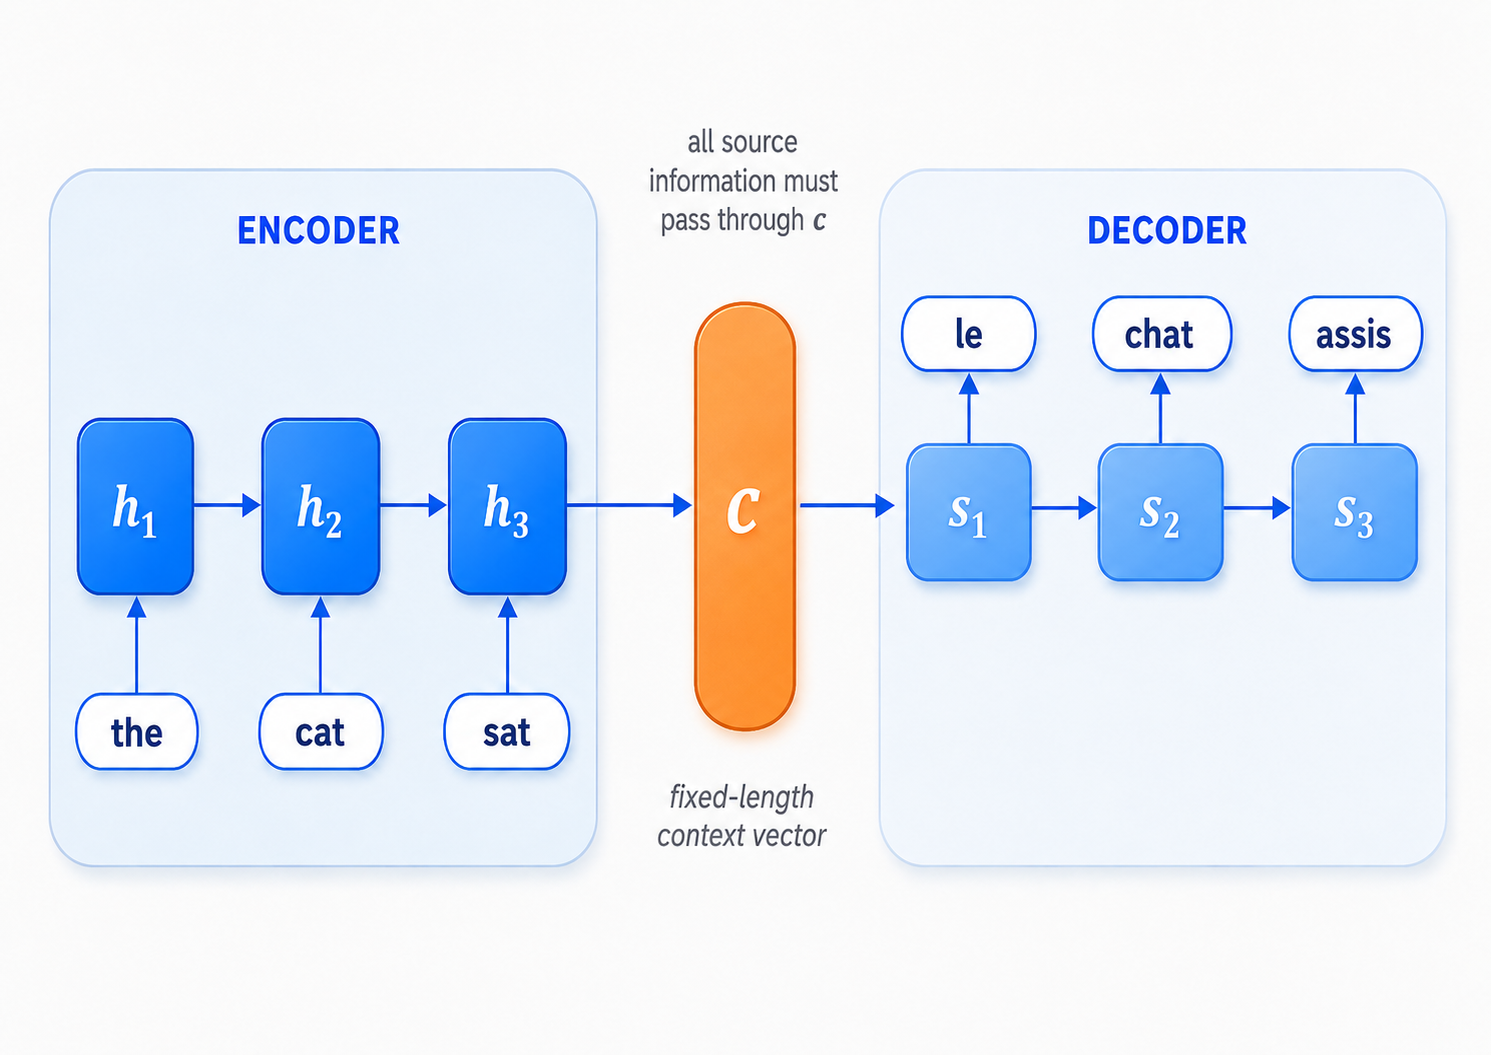
\includegraphics[width=0.9\textwidth]{figures/ch01/seq2seq_bottleneck.png}
\caption{The encoder--decoder (Seq2Seq) architecture. The encoder compresses the entire source sequence into a fixed-length context vector $\mathbf{c}$, which is the sole information conduit to the decoder---a critical bottleneck for long sequences.}
\label{fig:seq2seq}
\end{figure}

\subsection{Teacher Forcing}

During training, the decoder receives the \emph{ground-truth} previous token $y_{t-1}^*$ rather than its own prediction. This is called \emph{teacher forcing}. It stabilizes training because errors do not compound across time steps. However, it creates a train--test mismatch: at inference time, the model must condition on its own (potentially incorrect) predictions, and errors can cascade.

Scheduled sampling~\cite{bengio2015scheduled} mitigates this by randomly replacing ground-truth inputs with model predictions during training, with increasing probability as training progresses.

\subsection{The Bottleneck Problem}

The fixed-length context vector $\mathbf{c}$ is the critical weakness of vanilla Seq2Seq. The entire source sentence---regardless of length---must be compressed into a single vector of fixed dimension. For short sentences, this works reasonably well. For longer sentences, information is inevitably lost, and translation quality degrades sharply.

This bottleneck motivated the development of attention mechanisms.

\begin{quickrecap}
\textbf{Quick Recap.}
\begin{itemize}[nosep,leftmargin=1.5em]
  \item Encoder--decoder compresses the entire source into a single fixed-length vector---information bottleneck for long sequences.
  \item The 5th word and the 50th word compete for the same limited capacity.
  \item Teacher forcing stabilizes training but introduces exposure bias at inference.
\end{itemize}
\end{quickrecap}

\section{Early Attention Mechanisms}

\subsection{Bahdanau Attention}

Bahdanau et al.~\cite{bahdanau2015neural} proposed \emph{additive attention} to replace the fixed context vector with a dynamic, position-dependent summary. Instead of compressing the source into a single vector, the model retains all encoder hidden states $\mathbf{h}_1^{\text{enc}}, \ldots, \mathbf{h}_S^{\text{enc}}$ and computes a weighted combination at each decoder step:

\begin{align}
e_{t,s} &= \mathbf{v}^\top \tanh(\mathbf{W}_1 \mathbf{h}_s^{\text{enc}} + \mathbf{W}_2 \mathbf{h}_t^{\text{dec}}) \\
\alpha_{t,s} &= \frac{\exp(e_{t,s})}{\sum_{s'} \exp(e_{t,s'})} \\
\mathbf{a}_t &= \sum_{s=1}^{S} \alpha_{t,s}\, \mathbf{h}_s^{\text{enc}}
\end{align}

Here, $e_{t,s}$ is the \emph{alignment score} between decoder state $t$ and encoder state $s$, $\alpha_{t,s}$ is the attention weight (a probability distribution over source positions), and $\mathbf{a}_t$ is the context vector specific to decoder step $t$.

This was a breakthrough: instead of forcing all information through a single bottleneck, the decoder could ``look back'' at different parts of the source sentence at each generation step. Attention patterns often aligned with human intuitions about word alignment in translation.

\paragraph{A toy example.} Suppose we are translating ``the cat sat'' into French, and the decoder is about to generate the second target token. If the alignment scores are $e_{2,1} = 1.0$, $e_{2,2} = 3.5$, $e_{2,3} = 0.2$, then after softmax the attention weights are approximately $\alpha_{2,1} = 0.05$, $\alpha_{2,2} = 0.91$, $\alpha_{2,3} = 0.04$. The context vector $\mathbf{a}_2$ is dominated by the encoder state for ``cat''---the decoder is ``looking at'' the right source word for generating ``chat.'' The attention weight matrix across all decoder steps forms a soft alignment table between source and target.

\begin{figure}[ht]
\centering
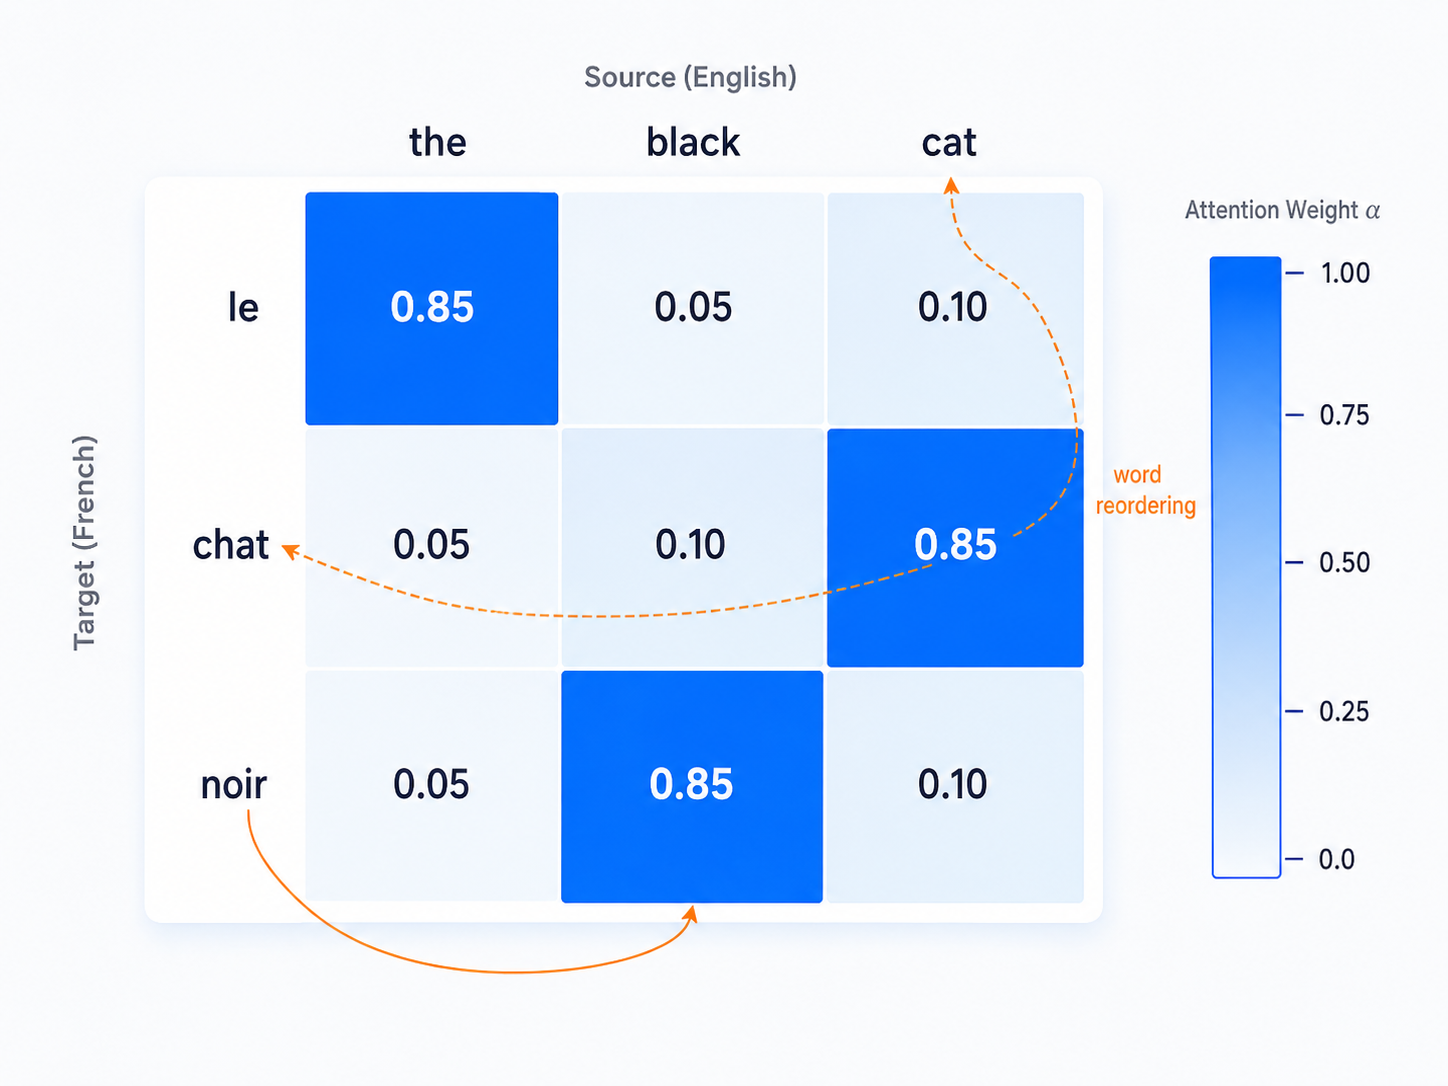
\includegraphics[width=0.75\textwidth]{figures/ch01/attention_heatmap.png}
\caption{Attention weights for a translation example. Each row shows where the decoder ``looks'' in the source sentence when generating each target word. A near-diagonal pattern indicates monotonic alignment; deviations indicate reordering.}
\label{fig:attention-heatmap}
\end{figure}

\subsection{Luong Attention}

Luong et al.~\cite{luong2015effective} simplified the scoring function. Instead of a learned feedforward network, they used a simple dot product:
\[
e_{t,s} = (\mathbf{h}_t^{\text{dec}})^\top \mathbf{h}_s^{\text{enc}},
\]
or a bilinear form $e_{t,s} = (\mathbf{h}_t^{\text{dec}})^\top \mathbf{W} \mathbf{h}_s^{\text{enc}}$. Dot-product attention is faster to compute and became the basis for the Transformer's scaled dot-product attention.

\subsection{Attention as a Differentiable Memory}

At a higher level, attention can be understood as a differentiable addressing mechanism over a memory bank (the encoder states). The decoder issues a ``query'' (its current state), computes similarity with all ``keys'' (the encoder states), and retrieves a weighted ``value'' (also the encoder states, in this formulation). This query--key--value framing, made explicit by the Transformer, is latent in Bahdanau and Luong attention.

To be precise: in Bahdanau attention, the decoder hidden state $\mathbf{h}_t^{\text{dec}}$ acts as the \emph{query}, while the encoder hidden states $\mathbf{h}_1^{\text{enc}}, \ldots, \mathbf{h}_S^{\text{enc}}$ serve as both \emph{keys} and \emph{values}. The Transformer generalizes this in two ways: first, it uses learned linear projections to create \emph{separate} key, value, and query representations, so keys and values are no longer forced to be the same vectors; second, it applies attention \emph{within} a single sequence (self-attention), not just between encoder and decoder. This second innovation---self-attention---is what ultimately eliminates the need for recurrence.

\medskip
\noindent\fbox{\parbox{\dimexpr\textwidth-2\fboxsep-2\fboxrule\relax}{\textbf{Pause and verify.} Bahdanau attention lets the decoder look at all encoder states. Does this also solve the \emph{encoder's} limitation of sequential computation? Why or why not?}}
\medskip

\begin{quickrecap}
\textbf{Quick Recap.}
\begin{itemize}[nosep,leftmargin=1.5em]
  \item Attention replaces the fixed bottleneck with a dynamic weighted sum over encoder states.
  \item Solves the information bottleneck: decoder ``looks back'' at different source positions each step.
  \item Does \emph{not} solve the sequential bottleneck---the encoder is still an RNN processing tokens one by one.
  \item The Q/K/V framing latent in Bahdanau attention becomes explicit in the Transformer.
\end{itemize}
\end{quickrecap}

\section{Autoregressive Generation Before Transformers}

All the models described so far generate text autoregressively: each token is produced conditioned on all previous tokens. The generation process is:

\begin{enumerate}
    \item Initialize the decoder state (from the encoder, or from a start token for unconditional generation).
    \item At each step, compute the distribution $P(w_t \mid w_{<t})$.
    \item Sample or select the next token.
    \item Feed the token back as input to the next step.
    \item Repeat until an end-of-sequence token is produced or a maximum length is reached.
\end{enumerate}

\textbf{Greedy decoding} selects $\arg\max P(w_t \mid w_{<t})$ at each step. It is fast but often produces repetitive or suboptimal sequences because a locally optimal choice at each step does not guarantee a globally optimal sequence.

\textbf{Beam search} maintains the top-$k$ partial sequences at each step, expanding each by one token and keeping the $k$ highest-scoring extensions. It produces better sequences than greedy decoding but is still deterministic and tends toward short, high-frequency outputs.

\textbf{Sampling} draws from the full distribution $P(w_t \mid w_{<t})$. Temperature scaling, top-$k$ truncation, and nucleus (top-$p$) sampling offer different ways to control the diversity--quality tradeoff. These same techniques---temperature, top-$k$, and nucleus sampling---are used in every modern LLM, from GPT-4 to LLaMA.

\section{Limitations of Recurrent Architectures}

By 2016--2017, RNN-based models with attention were the state of the art for machine translation and language modeling. But several fundamental problems remained:

\begin{enumerate}
    \item \textbf{Sequential computation.} The hidden state $\mathbf{h}_t$ depends on $\mathbf{h}_{t-1}$, which depends on $\mathbf{h}_{t-2}$, and so on. This sequential dependency means that the computation for a sequence of length $T$ requires $O(T)$ serial steps that cannot be parallelized across time. On modern GPUs, which excel at parallel matrix operations, this is a severe bottleneck for both training and inference.

    \item \textbf{Long-range dependencies in practice.} Despite the theoretical ability of LSTMs to carry information over long distances, empirical studies showed that effective context length was typically 100--200 tokens. Beyond that, even LSTMs struggled to maintain relevant information in their hidden state.

    \item \textbf{Limited direct interaction.} In an RNN, the representation of token $t$ can only interact with token $t'$ through the chain of hidden states between them. Information must pass through every intermediate step, being compressed and potentially corrupted at each one. There is no direct pathway from position 1 to position 100.

    \item \textbf{Attention was added on top, not built in.} In Bahdanau-style models, attention is applied between the encoder and decoder, but the encoder itself is still a sequential RNN. Self-attention---where every position attends to every other position within the same sequence---had not yet been explored as the primary computation mechanism.
\end{enumerate}

These limitations set the stage for the Transformer: an architecture where self-attention replaces recurrence entirely, enabling parallel computation over the full sequence and direct interaction between any two positions.

\begin{quickrecap}
\textbf{Quick Recap.}
\begin{itemize}[nosep,leftmargin=1.5em]
  \item Core limitation of RNNs is parallelism, not accuracy: hidden-state dependencies force $O(T)$ serial steps.
  \item Even with attention, the RNN encoder remains sequential---cannot saturate GPUs.
  \item These constraints, not benchmark performance, made the Transformer necessary.
\end{itemize}
\end{quickrecap}

\subsection{From Sequential Bottleneck to Parallel Attention}

The shift from sequential to parallel computation was not merely an engineering optimization---it changed what was scientifically feasible. Consider training a language model on 300 billion tokens. With an RNN, each token must be processed sequentially within each sequence, limiting throughput to the speed of serial matrix-vector operations. With a Transformer, all positions within a sequence are processed simultaneously, and throughput scales with the number of parallel cores.

This difference is what made large-scale pretraining practical. The GPT and BERT models that launched the modern era of language modeling were only possible because Transformer self-attention allowed efficient utilization of hundreds or thousands of GPUs. The architectural innovation of the Transformer is inseparable from the computational economics that enabled scaling.

\begin{figure}[h]
\centering
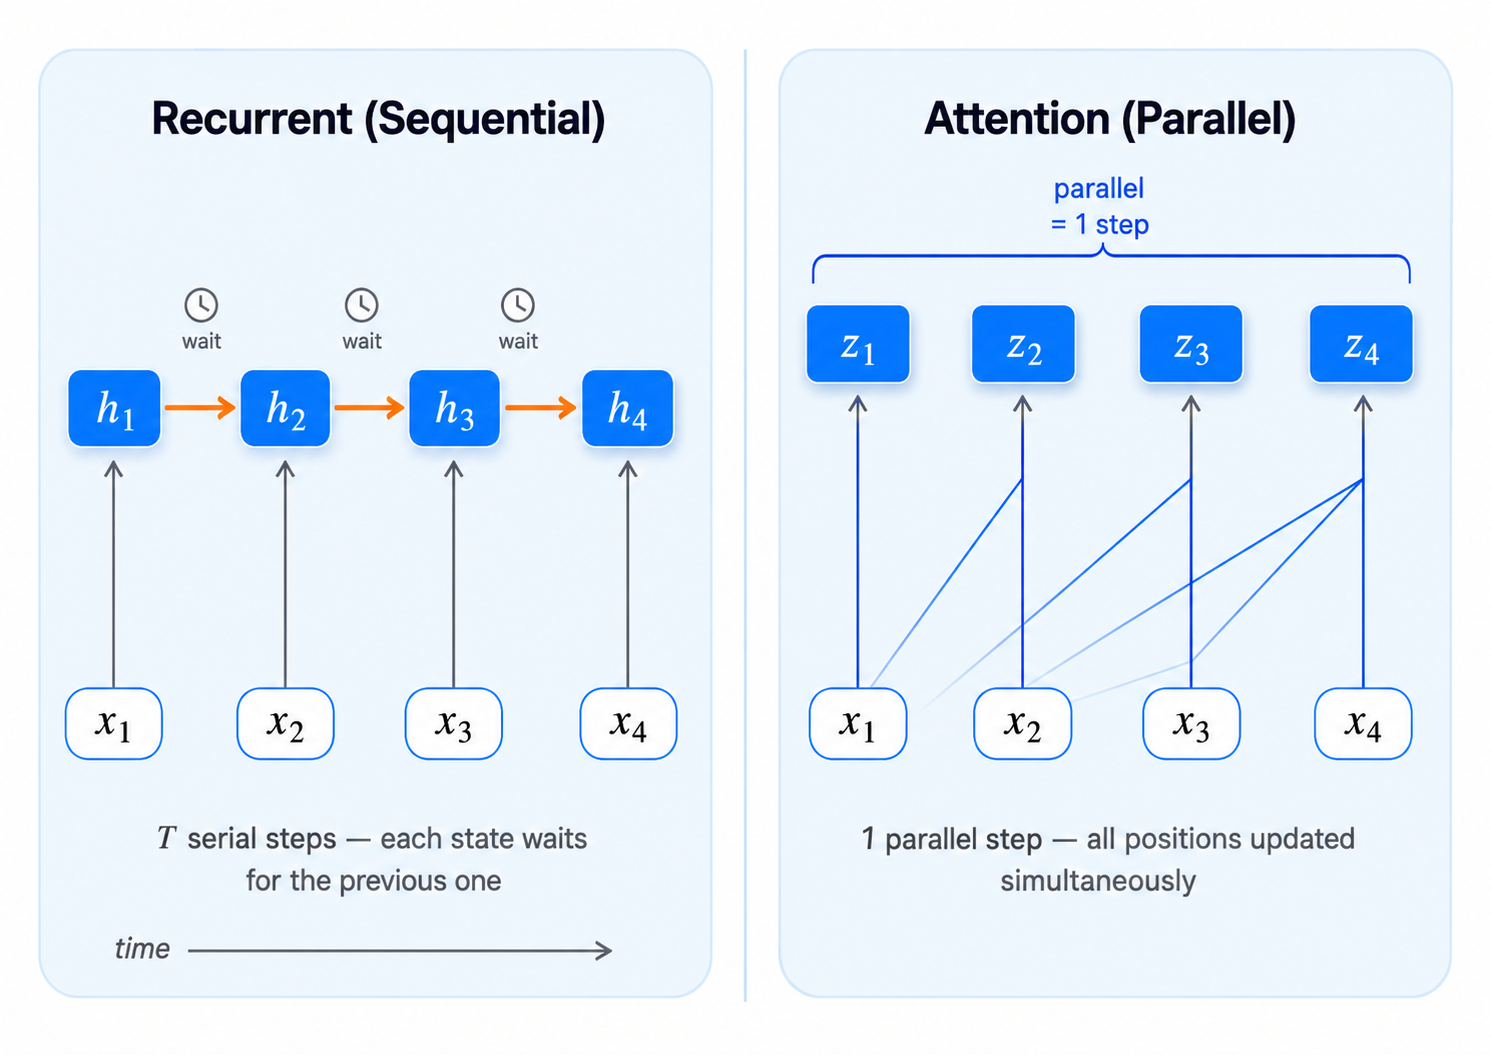
\includegraphics[width=0.9\textwidth]{figures/ch01/sequential_vs_parallel.png}
\caption{The fundamental computational difference between recurrent and attention-based architectures. \textbf{Left:} In an RNN, each hidden state $h_t$ must wait for $h_{t-1}$ to be computed, creating a serial chain of $T$ steps that cannot be parallelized across time. \textbf{Right:} In a Transformer layer, all positions are updated simultaneously through attention---each token directly accesses every other visible token in a single parallel step. This removal of time-wise recurrence is what enables efficient GPU utilization and makes large-scale pretraining practical.}
\label{fig:sequential-vs-parallel}
\end{figure}

\section{Trick Table}

The following techniques are operationally critical for working with pre-Transformer sequence models. Each one is something a first-year PhD student might reach for in a first experiment---and get burned by if they do not understand the failure mode.

\noindent
\begin{tabularx}{\textwidth}{@{}>{\raggedright\arraybackslash}p{2.8cm}
                              >{\raggedright\arraybackslash}p{2.8cm}
                              >{\raggedright\arraybackslash}p{3.2cm}
                              X@{}}
\toprule
\textbf{Trick} & \textbf{When to use} & \textbf{Expected effect} & \textbf{Failure signal} \\
\midrule
Gradient clipping &
  RNN/LSTM training; grad norm $> 5$--$10$ &
  Prevents exploding gradients; stabilizes training &
  Loss plateaus or diverges if clip threshold too small \\[4pt]
Truncated BPTT (seq.\ length) &
  Any recurrent model; typical range 64--256 &
  Controls memory cost and effective context length &
  Too short: loses long-range dependencies. Too long: OOM or slow convergence \\[4pt]
Hidden-state detach &
  Between truncated BPTT segments &
  Prevents gradient leaking across segments; bounds memory &
  Computation graph grows every batch; OOM after a few hundred steps \\[4pt]
Teacher forcing decay &
  Seq2Seq training &
  Reduces exposure bias by mixing in model predictions &
  Too fast: training instability. Too slow: no benefit until late \\[4pt]
Temperature / top-$p$ sampling &
  Text generation at inference &
  Controls diversity--quality tradeoff &
  High temp: incoherent. Low temp: degenerate repetition. Small $p$: overconfident \\
\bottomrule
\end{tabularx}

\section{Failure Modes and Common Misconceptions}

Before summarizing, let us address four misconceptions that commonly arise from a first reading of this material. Getting these right now will prevent confusion in later chapters.

\begin{itemize}
    \item \textbf{``RNNs cannot model long-range dependencies.''} This is an overstatement. LSTMs can maintain information over surprisingly long distances in controlled settings. The problem is that they do so unreliably: as sequence length increases, the probability of successfully retaining a specific piece of information decreases, and there is no mechanism for the model to ``decide'' in advance what to remember.

    \item \textbf{``Attention solved the bottleneck problem.''} Bahdanau attention solved the \emph{encoder--decoder} bottleneck but did not address the sequential computation bottleneck or the lack of direct within-sequence interaction. Those problems required self-attention and the removal of recurrence.

    \item \textbf{``N-grams are obsolete.''} For certain applications---especially low-resource settings, real-time systems, and interpretability---$n$-gram models or $n$-gram-augmented models remain practical. Understanding them is not just historical curiosity.

    \item \textbf{``Word2Vec embeddings are outdated.''} The \emph{specific} Word2Vec vectors are rarely used today, but the principle---learning distributed representations from co-occurrence patterns---is the foundation of every embedding layer in every neural language model.
\end{itemize}

\begin{takeaways}
\begin{itemize}[leftmargin=1.2em, itemsep=4pt]
  \item The recurring question is how models represent and use context: autoregressive LMs estimate $P(w_t \mid \text{context})$, while embedding methods use context as a training signal to learn reusable word vectors.
  \item Word2Vec is \emph{contextual in its training signal but static in its representation}: every occurrence of a word maps to the same vector regardless of sentence context.
  \item LSTM's cell state provides a \textbf{gradient highway}—when the forget gate is near 1, gradients flow backward through time almost unattenuated, which is why LSTMs handle long-range dependencies far better than vanilla RNNs.
  \item Gates are not hand-designed rules; they are differentiable control functions learned indirectly through prediction loss.
  \item The Seq2Seq bottleneck forced \emph{all} source information through a single fixed-length vector. Attention solved this by letting the decoder look back at every encoder state—but it did not solve the sequential computation bottleneck.
  \item Perplexity is the exponentiated empirical cross-entropy of the model on real text, not the intrinsic entropy of language.
  \item The fundamental limitation of recurrent models is not accuracy but \textbf{parallelism}: sequential hidden-state updates cannot saturate modern GPUs, which is what motivated the Transformer.
\end{itemize}
\end{takeaways}

\section{Summary}

\paragraph{Unifying view.} The recurring question in this chapter is how a model should represent and use context. Autoregressive language models make this explicit as $P(w_t \mid \text{context})$, while embedding methods such as Word2Vec and GloVe use context as a training signal to learn reusable word representations. What changed across generations was how context was represented, compressed, and accessed:

\begin{center}
\begin{tabularx}{\textwidth}{@{}lX@{}}
\toprule
Model & Context representation \\
\midrule
$N$-gram & Fixed symbolic window of $n{-}1$ tokens; raw counts \\
MLP Neural LM & Fixed window of embedding vectors; feedforward projection \\
RNN / LSTM / GRU & Variable-length history compressed into a recurrent hidden state \\
Seq2Seq + Attention & Dynamic, position-dependent weighted sum over encoder states \\
Transformer & Direct attention-based access to all positions; no recurrence \\
\bottomrule
\end{tabularx}
\end{center}

\noindent The history of language modeling before Transformers is the history of learning how to represent context: from fixed counts, to static vectors, to recurrent memory, to gated memory, and finally to direct attention.

\medskip
This chapter traced the evolution of sequence modeling through four generations:

\begin{enumerate}
    \item \textbf{N-gram models:} established autoregressive factorization and perplexity evaluation, but could not generalize beyond observed $n$-grams.
    \item \textbf{Distributed representations:} showed that words can be represented as dense vectors encoding semantic similarity, enabling generalization across similar contexts.
    \item \textbf{Recurrent networks:} provided variable-length context through hidden states, but suffered from vanishing gradients and sequential computation.
    \item \textbf{Attention:} allowed dynamic, position-dependent context aggregation, but was initially added on top of recurrent architectures rather than replacing them.
\end{enumerate}

Each generation solved problems left open by its predecessor, and each left problems that motivated the next. The Transformer, which we cover in Chapter~\ref{ch:attention}, takes the final step: replacing recurrence entirely with self-attention, enabling parallel computation, direct long-range interaction, and the scaling that produced modern large language models.

\medskip
\noindent\textit{Self-check: before moving to Chapter~\ref{ch:attention}, revisit the Learning Objectives at the start of this chapter. Can you address each one from memory, without scrolling back? If any point feels uncertain, re-read the corresponding section before continuing.}

\section*{Key Equations at a Glance}

\begin{center}
\renewcommand{\arraystretch}{1.6}
\begin{tabular}{lp{0.7\textwidth}}
\toprule
Model & Equation \\
\midrule
$N$-gram & $P(w_t \mid w_{t-n+1:t-1}) = \dfrac{\text{count}(w_{t-n+1:t})}{\text{count}(w_{t-n+1:t-1})}$ \\[4pt]
Perplexity & $\text{PPL} = \exp\!\bigl(-\tfrac{1}{T}\sum_{t=1}^T \log P(w_t \mid w_{<t})\bigr)$ \\[4pt]
RNN & $\mathbf{h}_t = \tanh(\mathbf{W}_h \mathbf{h}_{t-1} + \mathbf{W}_x \mathbf{x}_t + \mathbf{b})$ \\[4pt]
LSTM cell update & $\mathbf{c}_t = \mathbf{f}_t \odot \mathbf{c}_{t-1} + \mathbf{i}_t \odot \tilde{\mathbf{c}}_t$ \\[4pt]
LSTM hidden state & $\mathbf{h}_t = \mathbf{o}_t \odot \tanh(\mathbf{c}_t)$ \\[4pt]
GRU & $\mathbf{h}_t = (1-\mathbf{z}_t)\odot \mathbf{h}_{t-1} + \mathbf{z}_t \odot \tilde{\mathbf{h}}_t$ \\[4pt]
Bahdanau attention & $\mathbf{a}_t = \sum_s \alpha_{t,s}\,\mathbf{h}_s^{\text{enc}}, \quad \alpha_{t,s} = \text{softmax}(e_{t,s})$ \\
\bottomrule
\end{tabular}
\end{center}

\section*{Lab 1: Why Context and Gating Matter}

\subsection*{Goal}

This lab is the experimental companion to Chapter~1. Its purpose is not to build models from scratch, but to \emph{verify through experiment} the core claims of this chapter: that static embeddings collapse word senses, that vanilla RNNs fail on long-range dependencies due to gradient pathology, that LSTM gating solves this, that GRU achieves similar results with less overhead, and that attention removes the Seq2Seq bottleneck. You will use an AI coding assistant as your implementation partner---the skill being trained is experimental design and diagnosis.

\subsection*{Expected Time}

Day~2 (Experiments~0--3): 5--6 hours. Day~3 (Experiment~4 + Report): 4--5 hours.

\subsection*{Setup}

See \texttt{labs/ch01/README.md} for the full specification. You will need:
\begin{itemize}[nosep]
    \item A character-level language model supporting RNN, LSTM, and GRU (switchable via config).
    \item A synthetic delayed-memory task for controlled dependency-length testing.
    \item A minimal Seq2Seq model (with and without attention) for the bottleneck experiment.
    \item Pre-trained GloVe vectors (\texttt{glove.6B.100d}) for the embedding probe.
\end{itemize}
This is a \textbf{starter-code lab}: use an AI assistant to generate implementations from the specs in \texttt{labs/ch01/README.md}. Your time should go into running experiments, interpreting results, and writing the report---not fighting dataloaders or device placement. The code must be yours to understand and modify, but building it is not the bottleneck.

\subsection*{Verify}

Before running experiments, confirm these sanity checks on your char-level LM baseline:
\begin{enumerate}[nosep]
    \item \textbf{Hidden-state detach.} Confirm \texttt{hidden = tuple(x.detach() for x in hidden)} is called between BPTT segments. GPU memory and step time should remain constant across batches.
    \item \textbf{Loss alignment.} Feed a known short string (e.g., \texttt{"hello"}) and verify that the loss at position $t$ corresponds to predicting the character at position $t+1$.
    \item \textbf{Gradient logging.} Verify that gradient norms are being recorded at every step (before clipping). Plot a few hundred steps and confirm the values are reasonable (not all zeros, not NaN).
\end{enumerate}

\subsection*{Experiment 0: Static Embedding Polysemy Probe}

\textbf{Corresponds to:} \S\ref{sec:contextual-preview}, \S1.3.

\textbf{Goal:} See with your own eyes that a static embedding collapses multiple word senses into one vector.

\begin{enumerate}[nosep]
    \item Load pre-trained GloVe vectors (\texttt{glove.6B.100d}).
    \item Pick 3 polysemous words: \texttt{bank}, \texttt{cell}, \texttt{spring}.
    \item For each, find the top-10 nearest neighbors by cosine similarity.
    \item Classify each neighbor by which sense it belongs to (e.g., \texttt{bank}: financial vs.\ river edge).
    \item Run the analogy test: $\text{king} - \text{man} + \text{woman} \approx \text{queen}$.
\end{enumerate}

\textbf{What to look for:} Do nearest neighbors mix senses? If the \texttt{bank} neighbors are mostly financial, try other polysemous words or a different embedding. The key question is whether \emph{any} single vector can cleanly represent a word with multiple distinct meanings.

\textbf{Report:} For each polysemous word, list the top-10 neighbors and annotate which sense each belongs to.

\subsection*{Experiment 1: Gradient Pathology}

\textbf{Corresponds to:} \S1.4.1--1.4.3 (vanishing/exploding gradients, LSTM gradient highway).

\textbf{Goal:} Demonstrate that vanilla RNNs suffer from gradient instability, and that LSTM/GRU gating stabilizes training.

\begin{enumerate}[nosep]
    \item Train a vanilla RNN, LSTM, and GRU on the char-level LM task with \emph{identical} hyperparameters (hidden size, learning rate, batch size, sequence length).
    \item \textbf{Normal run:} gradient clipping enabled (max norm 5.0). Record gradient norm at every step for all three models. Plot gradient norm vs.\ step.
    \item \textbf{Stress run:} increase sequence length to 256, raise learning rate to 3e-3, \emph{disable} gradient clipping. Run for 500 steps. Record whether each model produces NaN loss, gradient spikes, or stable training.
\end{enumerate}

\textbf{What to look for:}
\begin{itemize}[nosep]
    \item Normal run: compare the variance and magnitude of gradient norms across models. Do gated architectures show more stable norms?
    \item Stress run: which model breaks first? If RNN does \emph{not} explode at these settings, increase learning rate or sequence length until you find its breaking point---characterize where the boundary lies. If LSTM also becomes unstable, note the conditions and compare thresholds.
\end{itemize}

\textbf{Report:} Gradient norm plots for all three models (normal run). One table summarizing the stress run outcome for each model.

\subsection*{Experiment 2: Long-Range Dependency Probe}

\textbf{Corresponds to:} \S1.4.1 (RNN captures short dependencies), \S1.4.3 (LSTM handles longer ones).

\textbf{Goal:} Show that RNNs can learn short-range patterns but fail at long range, while LSTMs retain information over longer distances.

\textbf{Task:} Synthetic delayed-memory. The model reads a sequence:
\[
\texttt{[marker]} \;\; a \;\; \texttt{[noise tokens} \times N\texttt{]} \;\; \texttt{[query]} \;\; \rightarrow \;\; a
\]
where $a$ is a random token placed after a marker, followed by $N$ noise tokens, then a query signal. The model must output $a$. This isolates dependency distance from all other confounds.

\begin{enumerate}[nosep]
    \item Train RNN, LSTM, and GRU on this task with dependency distances $N = 8, 32, 128, 256$.
    \item For each model $\times$ distance combination, record test accuracy after convergence.
    \item Plot accuracy vs.\ dependency distance for all three models on the same axes.
\end{enumerate}

\textbf{Training protocol:} Train separate models for each distance. This isolates the effect of dependency length from curriculum or mixed-difficulty effects. (Optional extension: train on mixed distances and test whether the model generalizes to longer unseen distances.)

\textbf{What to look for:}
\begin{itemize}[nosep]
    \item At what distance does each model's accuracy start to degrade? Is there a sharp cliff or a gradual decline?
    \item If results do not match predictions (e.g., RNN succeeds at $N = 128$), investigate: is the hidden size large enough to memorize? Is the task too easy? Adjust and rerun.
\end{itemize}

\textbf{Report:} One figure: accuracy vs.\ distance, three curves. One paragraph explaining why the results match (or don't match) the gradient highway theory from \S1.4.3.

\subsection*{Experiment 3: LSTM vs.\ GRU Efficiency}

\textbf{Corresponds to:} \S1.4.4 (GRU as simplified LSTM).

\textbf{Goal:} Quantify the efficiency--performance trade-off between LSTM and GRU.

\begin{enumerate}[nosep]
    \item From your Experiment 1 and 2 training runs, collect:
    \begin{itemize}[nosep]
        \item Parameter count (LSTM vs.\ GRU at same hidden size).
        \item Training throughput (tokens/sec or steps/sec).
        \item Final validation perplexity (char LM) or accuracy (delayed-memory task).
    \end{itemize}
    \item \textbf{Optional:} train GRU with a larger hidden size so that the parameter count matches LSTM. Compare convergence speed and final performance.
    \item Generate 200 characters from the trained LSTM and GRU (temperature 1.0) and qualitatively compare.
\end{enumerate}

\textbf{Report:} One table comparing parameters, throughput, and validation metric. One sentence on whether GRU achieves ``similar results with less overhead'' on these tasks, and any caveats.

\subsection*{Experiment 4: Seq2Seq Bottleneck and Attention}

\textbf{Corresponds to:} \S1.5--1.8 (Seq2Seq, attention, generation).

\textbf{Goal:} Show that compressing an entire input sequence into a single fixed-length vector creates a bottleneck that worsens with input length, and that attention solves this by letting the decoder access all encoder states.

\textbf{Task:} Sequence reversal. Input: \texttt{a b c d}, Output: \texttt{d c b a}. This task requires the decoder to access every encoder position---the first output token depends on the \emph{last} input token, making the bottleneck maximally visible.

\begin{enumerate}[nosep]
    \item Implement two models: (a) LSTM encoder-decoder \emph{without} attention (context = final encoder hidden state only), and (b) LSTM encoder-decoder \emph{with} Bahdanau attention.
    \item Train both models on the reverse task with input lengths $L = 10, 30, 50, 100$.
    \item For each model $\times$ length combination, record test accuracy (exact sequence match).
    \item Plot accuracy vs.\ input length for both models on the same axes.
    \item For the attention model at $L = 30$, visualize the attention weight matrix $[\alpha_{t,s}]$ for one example. Describe the pattern.
\end{enumerate}

\textbf{What to look for:}
\begin{itemize}[nosep]
    \item Without attention: at what length does accuracy start to collapse? Is the degradation gradual or sudden?
    \item With attention: does it maintain high accuracy at $L = 100$? If not, check training budget---attention models may need more epochs to converge on longer sequences.
    \item Attention heatmap: does the pattern resemble an anti-diagonal? If it is noisy, the model may need more training, or the attention mechanism may have a bug.
\end{itemize}

\textbf{Report:} One figure: accuracy vs.\ length, two curves. One attention heatmap. One paragraph connecting the results to the bottleneck discussion in \S1.5.

\subsection*{Optional Extensions}

\begin{enumerate}
    \item \tierstretch{} \textbf{Parameter-matched GRU.} Train GRU with a larger hidden size so its total parameter count matches LSTM. Does closing the parameter gap also close the performance gap?
    \item \tierstretch{} \textbf{Mixed-distance generalization.} Train one LSTM on a mixture of all dependency distances ($N = 8, 32, 128, 256$). Test on $N = 512$---a distance never seen during training. Does the model generalize, or does it fail on unseen distances?
    \item \tierstretch{} \textbf{Bidirectional encoder.} Replace the unidirectional encoder in Experiment~4 with a bidirectional LSTM. Does it improve accuracy on the no-attention model? On the attention model?
\end{enumerate}

\subsection*{Deliverables}

\begin{itemize}[nosep]
    \item Runnable code for all five experiments, with clear instructions.
    \item Verification notes: three sentences, one per sanity check.
    \item Figures: gradient norm plot (Exp~1), accuracy vs.\ distance (Exp~2), accuracy vs.\ length (Exp~4), attention heatmap (Exp~4).
    \item Tables: polysemy neighbors (Exp~0), efficiency comparison (Exp~3).
    \item A 500--700 word experiment report (see below).
\end{itemize}

\subsection*{Evaluation Rubric}

\begin{center}
\begin{tabular}{lp{0.7\textwidth}}
\toprule
Weight & Criteria \\
\midrule
15\% & Setup: all models train correctly; sanity checks pass. \\
20\% & Experiments 1--2: gradient and dependency results are measured carefully and used to analyze RNN limitations and LSTM/GRU improvements. \\
15\% & Experiment 3: efficiency comparison has quantitative data and honest interpretation. \\
20\% & Experiment 4: bottleneck clearly demonstrated; attention heatmap correctly interpreted. \\
20\% & Experiment report: causal reasoning connecting results to chapter theory. \\
10\% & Reproducibility: code, configs, and instructions sufficient for replication. \\
\bottomrule
\end{tabular}
\end{center}

\section*{Experiment Report}

Write a 500--700 word report structured around one question: \emph{which architectural change addressed which failure mode?}

\begin{description}[style=nextline, leftmargin=1.5em]
    \item[Question.] What failure mode does each architectural change address?
    \item[Evidence.] Summarize the key quantitative results from all five experiments. Use numbers and plots rather than vague impressions.
    \item[Diagnosis.] Connect each result to the theory from this chapter: static embeddings and polysemy, vanishing gradients, gated memory, GRU efficiency, and the Seq2Seq bottleneck.
    \item[Trade-offs.] What did GRU save compared with LSTM? What did attention fix that recurrence and gating alone did not?
    \item[Next step.] If you had one more day, what would you try next?
\end{description}

\noindent\textit{A strong report includes at least one result that surprised you and an honest explanation of what you do not yet understand. If you caught an implementation bug or a misleading suggestion during the lab, briefly describe how you identified it.}

\section*{Key Readings}

\nocite{bengio2003neural,mikolov2013efficient,pennington2014glove,hochreiter1997lstm,cho2014learning,sutskever2014sequence,bahdanau2015neural,luong2015effective,peters2018elmo,vaswani2017attention}

\begin{description}[style=nextline, leftmargin=1.5em]
    \item[Bengio et al.\ (2003). \normalfont\textit{A Neural Probabilistic Language Model.} JMLR.]
    Read for: the first neural language model---learned embeddings fed into a feedforward network for next-word prediction. Start here to understand why dense representations replaced counts.

    \item[Mikolov et al.\ (2013). \normalfont\textit{Efficient Estimation of Word Representations in Vector Space.}]
    Read for: Word2Vec (skip-gram and CBOW). Focus on negative sampling and the analogy experiments.

    \item[Pennington et al.\ (2014). \normalfont\textit{GloVe: Global Vectors for Word Representation.} EMNLP.]
    Read for: an alternative derivation of word embeddings from global co-occurrence statistics.

    \item[Hochreiter \& Schmidhuber (1997). \normalfont\textit{Long Short-Term Memory.} Neural Computation.]
    Read for: the gating mechanism that solved vanishing gradients. Focus on Section~3 (cell architecture) and Section~5 (experiments).

    \item[Cho et al.\ (2014). \normalfont\textit{Learning Phrase Representations using RNN Encoder--Decoder.} EMNLP.]
    Read for: the GRU architecture and the encoder--decoder framework. Shorter and more accessible than the LSTM paper.

    \item[Sutskever et al.\ (2014). \normalfont\textit{Sequence to Sequence Learning with Neural Networks.} NeurIPS.]
    Read for: the Seq2Seq paradigm at scale---deep LSTMs for translation without attention. Notice how reversing the source sequence hinted at the information bottleneck.

    \item[Bahdanau et al.\ (2015). \normalfont\textit{Neural Machine Translation by Jointly Learning to Align and Translate.} ICLR.]
    Read for: the attention mechanism that directly inspired the Transformer. The most important paper in this list---understand the alignment model, the context vector, and the attention visualizations.

    \item[Luong et al.\ (2015). \normalfont\textit{Effective Approaches to Attention-based Neural Machine Translation.} EMNLP.]
    Read for: the simplification from additive to dot-product attention---the basis for scaled dot-product attention in the Transformer.

    \item[Peters et al.\ (2018). \normalfont\textit{Deep Contextualized Word Representations.} NAACL.]
    Read for: ELMo---pretrained contextualized representations that transfer across tasks. The bridge from static embeddings to BERT/GPT.

    \item[Vaswani et al.\ (2017). \normalfont\textit{Attention Is All You Need.} NeurIPS.]
    Read for: the destination. Skim the architecture after this chapter; we cover it in detail in Chapter~\ref{ch:attention}. Note how every design choice responds to a limitation discussed above.
\end{description}

\bigskip
\noindent\textbf{What's next.}\quad Chapter~\ref{ch:attention} picks up exactly where this chapter ends: we dismantle the Transformer layer by layer---multi-head self-attention, positional encoding, layer normalization, and the feed-forward sub-network---and show how each component addresses the specific limitations identified here. If this chapter explained \emph{why} recurrence had to go, the next chapter shows \emph{what replaced it}.
